\subsection{Negativo da Imagem}

Para essa conversão basta fazer ~\pyline{255 - intensidade}~ para cada píxel. Como 255 também é o maior valor de um \textit{byte}, a operação é equivalente a inverter todos os bits da imagem.

\begin{figure}[H]
    \centering
    \begin{subfigure}{0.45\textwidth}
        \centering
        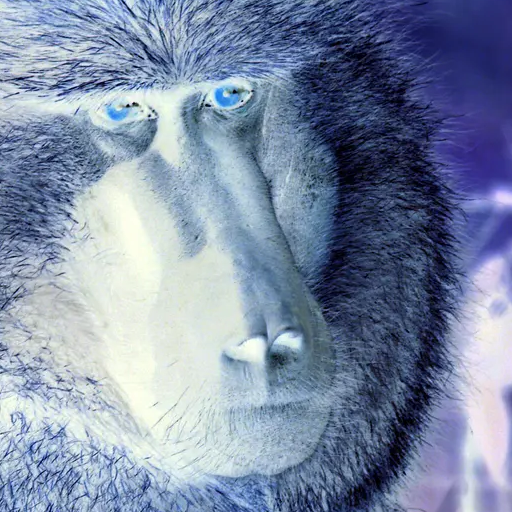
\includegraphics[width=6cm]{resultados/colorneg.png}
        \caption{\texttt{imagens/color.png}}
    \end{subfigure}%
    \begin{subfigure}{0.45\textwidth}
        \centering
        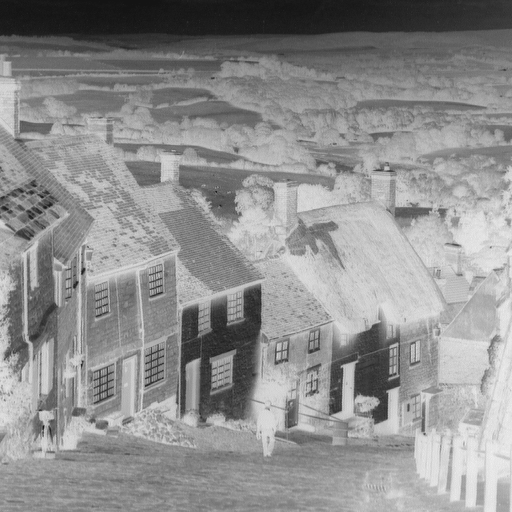
\includegraphics[width=6cm]{resultados/cityneg.png}
        \caption{\texttt{imagens/city.png}}
    \end{subfigure}

    \caption{Imagem com intensidade invertida.}
\end{figure}

\begin{listing}[H]
    \begin{minted}{python}
        def negativo(imagem):
            return ~imagem
    \end{minted}

    \caption{Comando \texttt{negativo}}
\end{listing}

Em vez de usar o \textit{not} (\pyline{~}) do \pyline{ndarray}, existe também a função \pyline{cv2.bitwise_not(imagem)} \autocite{ref:bitwise_not}.
